\section{Rešitev}

Najprej si poglejmo animacijo v mapi \verb|./latex/mp4/analytic_solution.mp4| in \verb|naive_aproach.mp4|.
Vidimo, da dela le približno pravilno.

\begin{figure}[h]
    \centering
    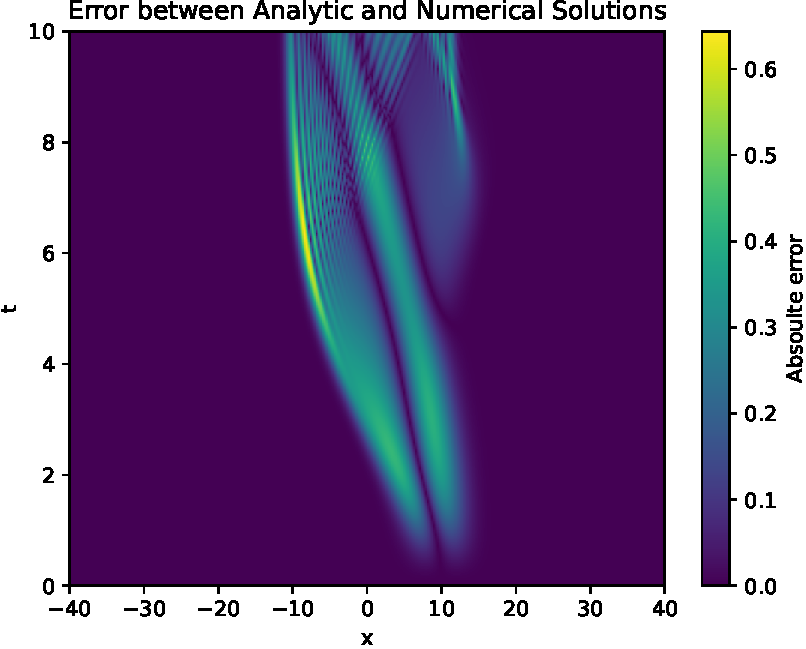
\includegraphics[width=0.4\textwidth]{pdf/abs_error.pdf}
    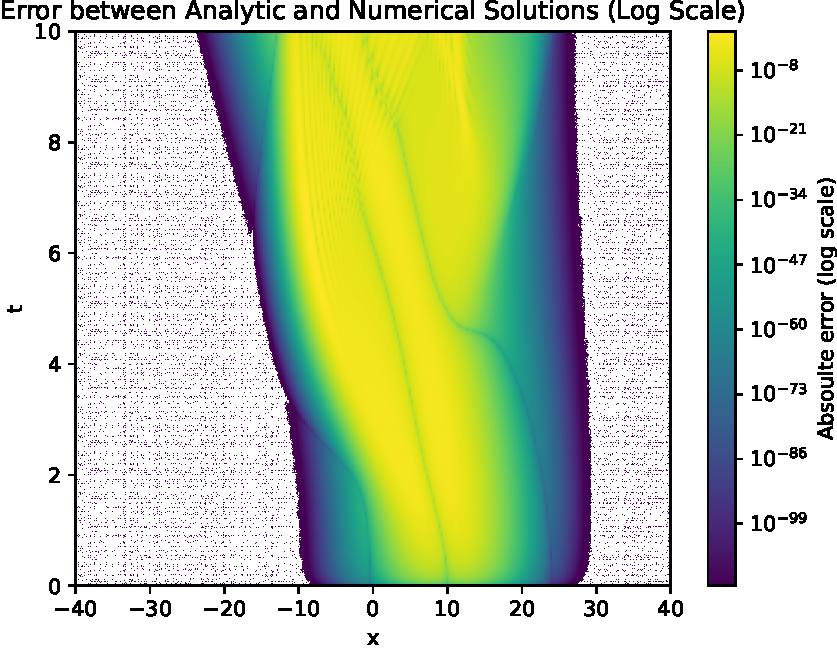
\includegraphics[width=0.4\textwidth]{pdf/abs_error_log.pdf}
    \caption{Absolutna napaka v odvisnosti od časa.}
\end{figure}
Poglejmo si, kako se napaka spreminja, če povečamo natančnost odvoda, z dodatnimi diagonalnimi členi.
\begin{figure}[h]
    \centering
    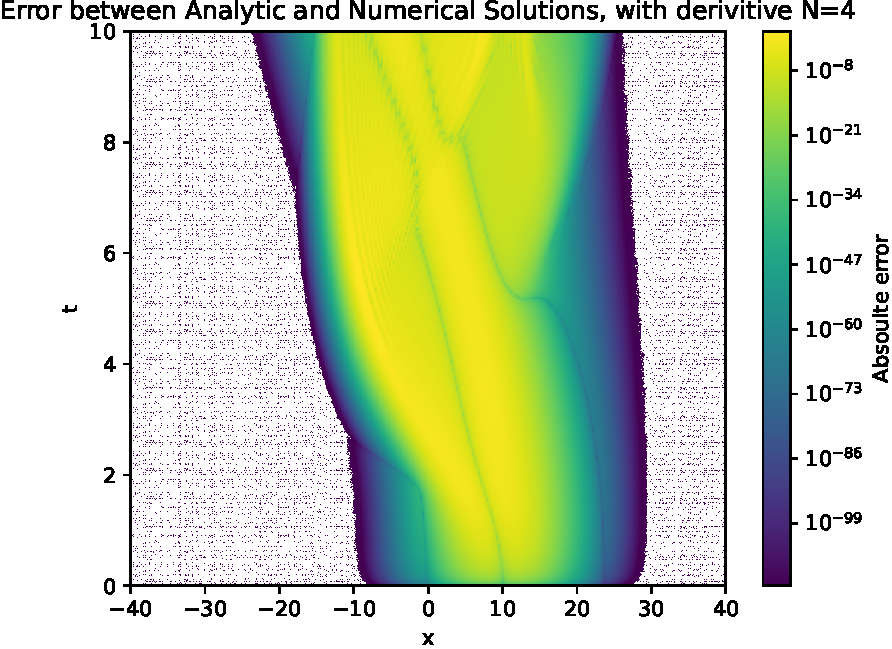
\includegraphics[width=0.4\textwidth]{pdf/abs_error_log_4.pdf}
    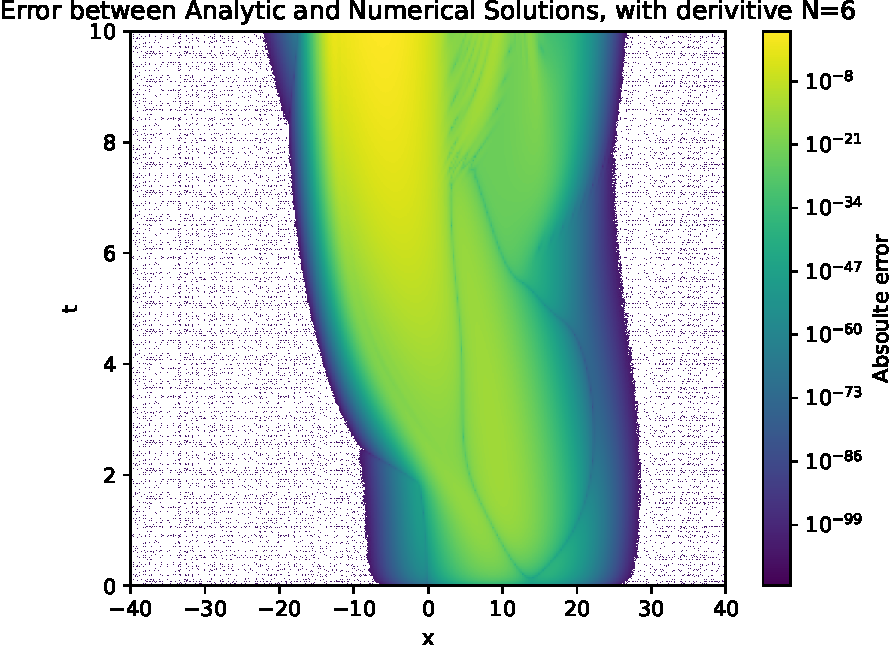
\includegraphics[width=0.4\textwidth]{pdf/abs_error_log_6.pdf}
    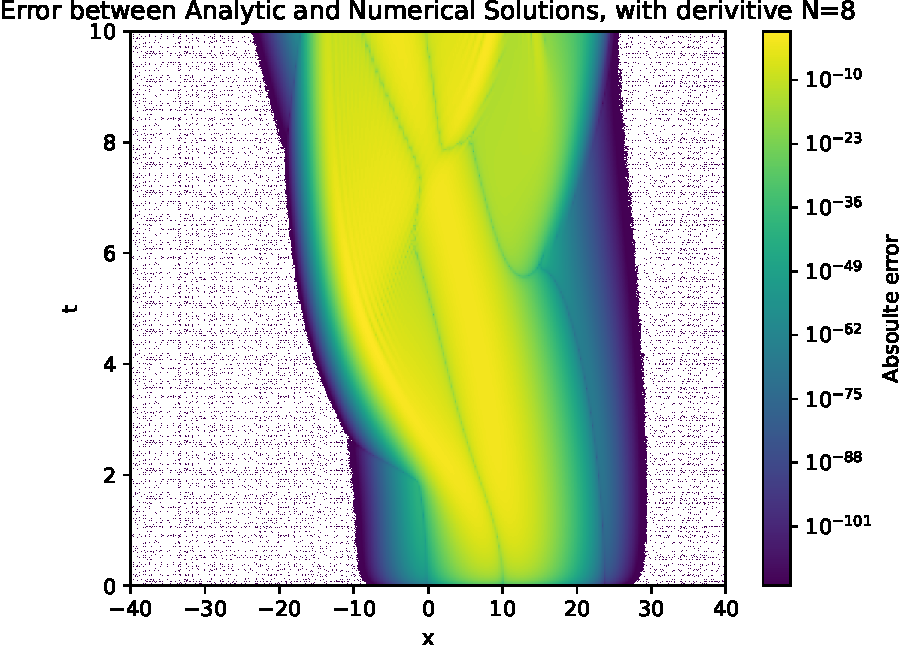
\includegraphics[width=0.4\textwidth]{pdf/abs_error_log_8.pdf}
    \caption{Odvisnost napake od natančnosti drugega odvoda}
\end{figure}
Absolutna napaka se zmanjšuje z večanjem natančnosti odvoda.
Kako se pa spreminja maksimum napake v odvisnosti natančnosti odvoda?
\newpage
\begin{figure}[h]
    \begin{center}
    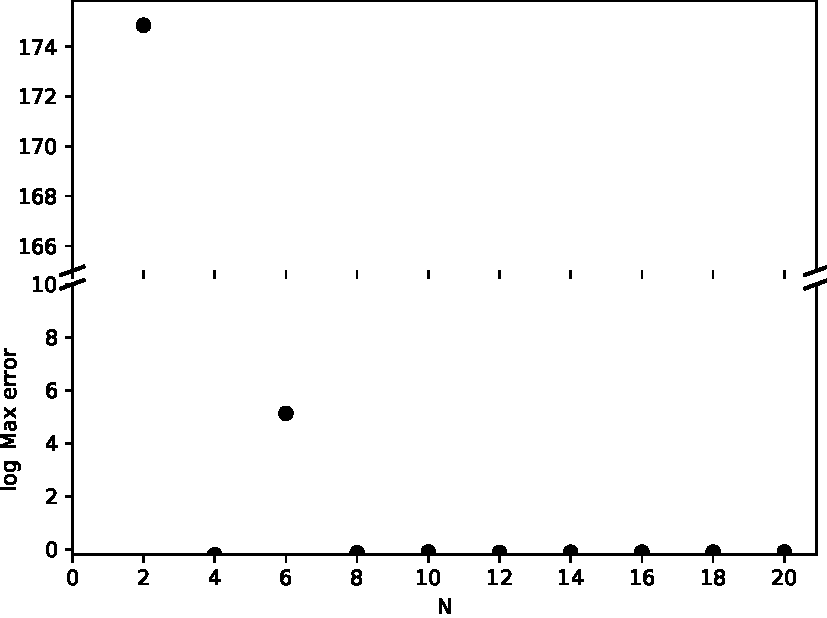
\includegraphics[width=0.4\textwidth]{pdf/max_error.pdf}
    \end{center}
    \caption{Maksimalna napaka v celotnem časovnem obdobju v odvisnosti od natančnosti drugega odvoda}
\end{figure}

Kako pa je z napako, če dodamo Padéjev približek?
\begin{figure}[h]
    \centering
    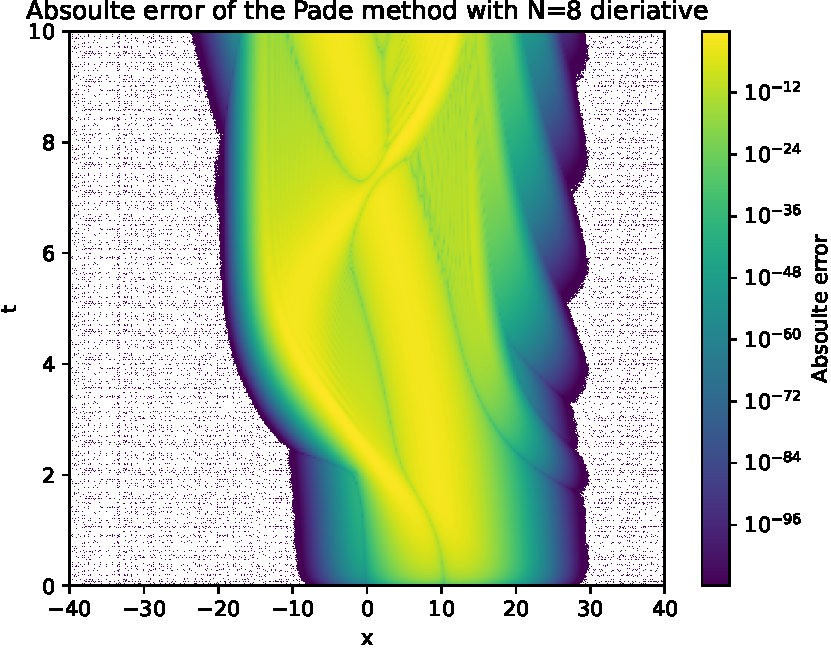
\includegraphics[width=0.4\textwidth]{pdf/abs_error_pade.pdf}
    \caption{Absolutna napaka v odvisnosti od časa z Padéjevim približkom reda $M=8$}
\end{figure}
Napaka se s časoma malo manj propagira. Iz slike, da popravek manj vpliva kot krajevna natančnost drugega odvoda.
S tem približkom smo dobili dva reda natančnosti.
\newpage

Poglejmo si še časovno analizo. Kot vemo se z obema približkoma spremeni le konstanta v big-$O$ notaciji.
\begin{figure}[h]
    \centering
    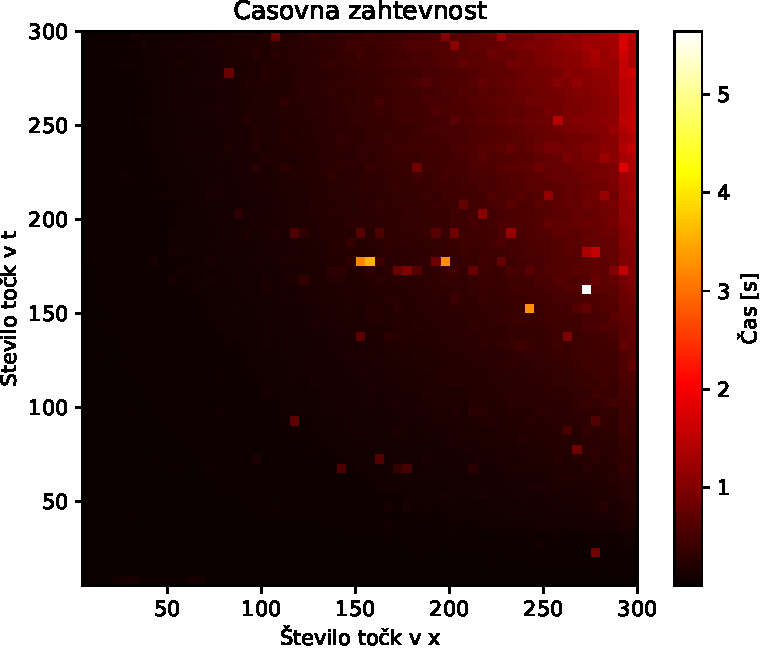
\includegraphics[width=0.4\textwidth]{pdf/time.pdf}
    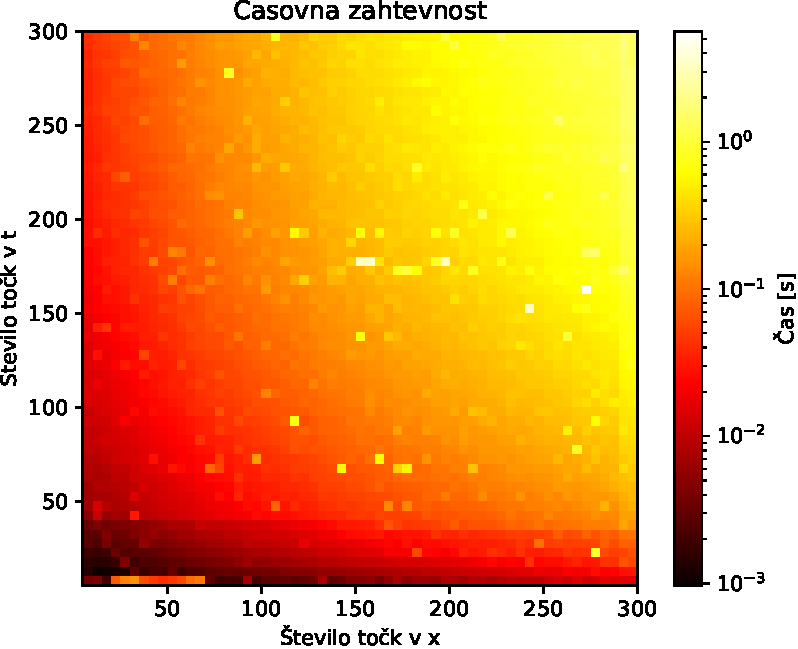
\includegraphics[width=0.4\textwidth]{pdf/time_log.pdf}
    \caption{Časovna analiza}
\end{figure}

Poglejmo si podrobneje kako se za nekatere fiksne vrednosti spreminja čas.
\begin{figure}[h]
    \centering
    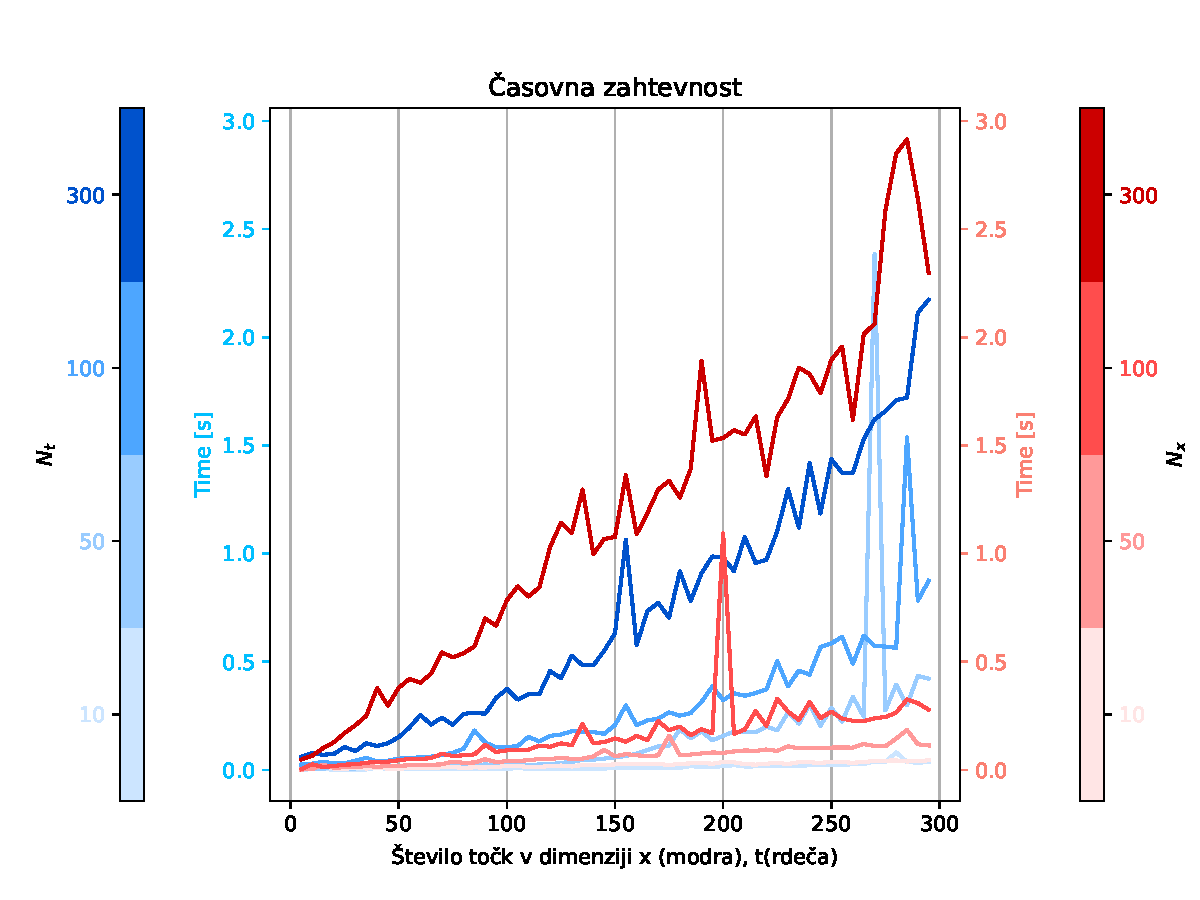
\includegraphics[width=0.8\textwidth]{pdf/time1.pdf}
    \caption{Časovna analiza za nekatere fiksne vrednosti}
\end{figure}
